\documentclass[preprint,10pt]{elsarticle}
\usepackage{etoolbox}
\makeatletter
\patchcmd{\ps@pprintTitle}{\footnotesize\itshape
       Preprint submitted to \ifx\@journal\@empty Elsevier
       \else\@journal\fi\hfill\today}{06.2018}{}{}
\makeatother

\usepackage[margin=2.5cm]{geometry}

\newcommand{\fscale}[1]{#1\linewidth}
\newcommand{\figref}[1]{Fig.~\ref{#1}}

%-----------------------------------------------------------------------------
%  Colors
%-----------------------------------------------------------------------------
\usepackage{pagecolor}
\definecolor{linen}{RGB}{240,240,230}
\definecolor{fwhite}{RGB}{255,250,240}
\definecolor{oldlace}{RGB}{253,245,230}
\definecolor{awhite}{RGB}{250,235,215}
\definecolor{pwhip}{RGB}{255,239,213}
\definecolor{peach}{RGB}{255,218,185}
\definecolor{ivory}{RGB}{255,255,240}
\definecolor{seashell}{RGB}{	255,245,238}

\usepackage{sectsty}
\sectionfont{\Large}
\subsectionfont{\large}

\usepackage{amsmath}
\newcommand{\mr}[1]{\mathrm{#1}}  % Roman font for the math mode
\newcommand{\mi}[1]{\mathit{#1}}  % Italic font for the math mode
\newcommand{\mc}[1]{\mathcal{#1}} % Caligrafic (script) font for the math mode
\newcommand{\ms}[1]{\mathsf{#1}}  % Sans font for the math mode (vectors and matrices)
\newcommand{\mb}[1]{\mathbf{#1}}  % Bold font for the math mode (vectors and matrices)

\usepackage{mathtools}
\DeclarePairedDelimiter\ceil{\lceil}{\rceil}
\DeclarePairedDelimiter\floor{\lfloor}{\rfloor}

\usepackage{amsthm}
\theoremstyle{definition}
\newtheorem{definition}{Definition}[section]
\newtheorem{remark}{Rule}[section]

\newtheorem{property}{Property}

\newtheorem{theorem}{Theorem}

\usepackage{cleveref}
\crefformat{section}{\textbf{\S#2#1#3}} % see manual of cleveref, section 8.2.1
\crefformat{subsection}{\textbf{\S#2#1#3}}
\crefformat{subsubsection}{\textbf{\S#2#1#3}}

\renewcommand{\cref}[1]{\textbf{\S\ref{#1}}}

\usepackage{graphicx}
\usepackage{subfigure}
\graphicspath{{./fig/}}
%% The amssymb package provides various useful mathematical symbols
\usepackage{amssymb}

\usepackage[titletoc]{appendix}
\usepackage[T1]{fontenc}

\usepackage{xcolor, soul}
\sethlcolor{oldlace}

\usepackage{lineno}
\usepackage{url}
\bibliographystyle{unsrt}

\patchcmd{\abstract}{Abstract}{Summary}{}{}

\begin{document}

\begin{frontmatter}

%% Title, authors and addresses

\title{Latitude: A Blockchain for the Transportation Industry\tnoteref{title1}}
\tnotetext[title1]{Version 1.1}

\author{Latitude Labs\corref{auth1}}
\cortext[auth1]{https://latitude0x.com}
\address{Bay Area, Silicon Valley, California}

\begin{abstract}

    Testing.
\newline
\newline
\newline
\newline
\end{abstract}

\begin{keyword}
	\textsf{decentralization \sep blockchain \sep ethereum \sep database \sep sql \sep access control \sep secret sharing \sep p2p \sep tokens \sep incentives \sep mechanism design \sep byzantine faults \sep data sharing}
\end{keyword}

\end{frontmatter}

\newpage
\tableofcontents
\newpage

%-----------------------------------------------------------------------------
%  INTRODUCTION
%-----------------------------------------------------------------------------
\section{Introduction}\label{sec:intro}

- There is a fundamental shift happening in the transportation industry. Automation, data, AI based analytics.
- Centralized solution examples:
    - Telematics data exchanges.
    - Mapping and location data: privacy security issues. Lack of user control.
    - Centralization creates DATA SILOS. Explain and expand.
- What powers this is data, being able to share data, analytics, computation using AI, in a trustworthy privacy-aware
manner.

- The industry needs a solution that can allow new ways of sharing the data while providing strong unbreakable gurantees
of security privacy etc.


- Overview of our solution:
  - Blockchains can provide these gurantees and much more. 
  - Examples of other industries where blockchain is posed to disrupt traditional data sharing:
    - IOT example.
    - Supply chain management.
    - Renting.
  - Section level overview.



We are in the midst of building a new Internet. Blockchain networks like Ethereum have popularized the idea of unstoppable, owner less applications that are run on an open network of untrusted but incentivized nodes without the oversight of a central authority. An increasing number of these decentralized applications (\DJ apps) are being created everyday with evolving data storage needs. The first generation of these dapps stored their data entirely on a blockchain itself while the current ones are storing it on decentralized file storage systems like IPFS with just hashes of the data stored on the blockchain. Although this method works for dapps with simple storage needs like the need for storing data as a blob, it is very limiting for dapps with more complex requirements such as the need to store data at a more fine grained level and efficiently querying it. A popular option is then to use a cloud hosted database (ex: Google’s Cloud SQL) but that turns a dapp into a non-dapp by introducing centrality into the system. \newline\newline

Rest of the paper is structured as follows: in section 2, we discuss some related work. Section 3 presents the overall design of the system, section 4 presents the network subsystem, section 5 presents the database subsystem and section 6 presents our approach to dealing with problems that arise in a network made up of untrusted nodes and discusses an incentive mechanism to make them behave as per system's needs. In section 7, we propose a message exchange protocol in the same vein as http but for relational data sharing. Section 8 concludes the paper.


The introduction of Bitcoin \cite{nakamoto2009bitcoin} has triggered a new wave of decentralization in computing. 
Bitcoin illustrated a novel set of benefits: decentralized control, where ``no one'' owns or controls the network; immutability,
where written data is tamper-resistant (``forever''); and the ability to create \& transfer assets on the network, without reliance on a central entity.

The initial excitement surrounding Bitcoin stemmed from its use as a token of value, for example as an alternative to government-issued currencies.
As people learned more about the underlying blockchain technology, they extended the scope of the technology itself (e.g. smart contracts), as well as applications (e.g. intellectual property).

With this increase in scope, single monolithic ``blockchain'' technologies are being re-framed and refactored into building blocks at four levels of the stack:
\begin{enumerate}
 \item Applications
 \item Decentralized computing platforms (``blockchain platforms'')
 \item Decentralized processing (``smart contracts'') and decentralized storage (file systems, databases), and decentralized communication
 \item Cryptographic primitives, consensus protocols, and other algorithms
\end{enumerate}




%-----------------------------------------------------------------------------
%  Blockchain SECTION
%-----------------------------------------------------------------------------
\section{Blockchain-based Approaches}\label{sec:blockchain}


\section{The Latitude Blockchain}\label{sec:design}


Overview of design principles:

Datastore
 - Optimized for Geographic, Geo-spatial data.
 - Location, Mapping data and computation.
 - Ability to Store, index, query and build smart contracts optimized for such data.
 - Support for various spatial indexes.
 - Location heatmaps.
 - Indexing road and driving data.
 - Primitives for storing driving data for autonomous vehicles

Cryptographic primitives for:
 - Security and privacy of data.
 - Anonymity guarantees using cryptographic set operations.
 - Enforcement of privacy when sharing data.
 - Sharing of “computation” instead of data when possible.
 - For eg: Sharing of DriverScore using a vetted algorithm.
 - Sharing proximity to a landmark instead of lat/lng.
 - Ability to find bad actors.
 - Detect privacy, anonymity and security violations.


Smart contract system for Transportation applications.
 - Ability to convert “policies” such as GDPR into smart contract code.
 - Example, self destruct data after a time period.
 - Sandboxed trusted execution environment:
 - For algorithms:
   - DriverScore, Location heatmaps, Statistics.
   - Enforcing or verifying privacy and other govt policies/regulations.

Cryptographic proofs for applications:
 - Proof of Location. 
 - Proof of ride. 
 - Proof of mapping 
      (road/landmark exists or does not exist).
 - Proof of driver score 
 - Open, trusted, understood driver score computation algorithms.
 - Cryptographic proofs can be shared among entities, safely, securely.


Cryptoeconomics and Governance:
 - Crypto-incentives for honest operation.
 - Penalties for malicious intent.
 - Governance based on consensus and roles using a council.
 - Council members elected using voting, stake and established trust.
 - Some council members can have restricted access.
 - Eg: US govt can have voting rights on US data/users, etc.

User incentives:
 - Users have full control over their data and computation.
 - Users can issue or request proofs to carry over to other applications.
 - User’s have incentive to share data, participate in improving the common denominator.
 - Malicious intent, Byzantine behavior.
   - Can be detected using a combination of consensus and incentives.
   - Best interest of users to act honestly by design.

\subsection{Blockchain Architecture}




\section{Applications}
\label{sec:apps}


\subsection{Rideshare applications}


\subsection{Telematics applications}

\subsection{Mapping and Location}

\subsection{Smart city and Govt Applications}


\section{Mechanism Design}
\label{sec:mech}


% One section per vertical.

% Core blockchain aspects. Smart Contract system. DataStore etc.

% Governance. Consensus, cryptoeconomics.

%-----------------------------------------------------------------------------
%  OVERALL DESIGN SECTION
%-----------------------------------------------------------------------------
%\section{The Latitude Blockchain}\label{sec:design}

In this section, we present a high-level design of the Latitude blockchain. The full-version of this whitepaper shall
contain a very detailed design of each component. We start with an overview of the key design principles that will guide
the rest of the design for the Latitude Blockchain. Its important to note here that for implementation purposes, it
might be possible to use an existing core blockchain for the underlying functionalities and build Latitude as a layer on
top. We shall make these determinations in the full-version of the whitepaper.

\subsection{Design overview}

The purpose of the Latitude blockchain is to become the best platform in the world for decentralized applications for
the Transportation Industry. Specifically, this boils down to constructs in the blockchain that can handle spatial,
mapping, traffic, driving data including data relating to other modalities of transport (bike sharing, walking, even air
routes later on). Figure XXX presents the architecture of the Latitude blockchain in terms of the core technological
innovations that will be built into it.

\begin{figure}[t]
    \centering
    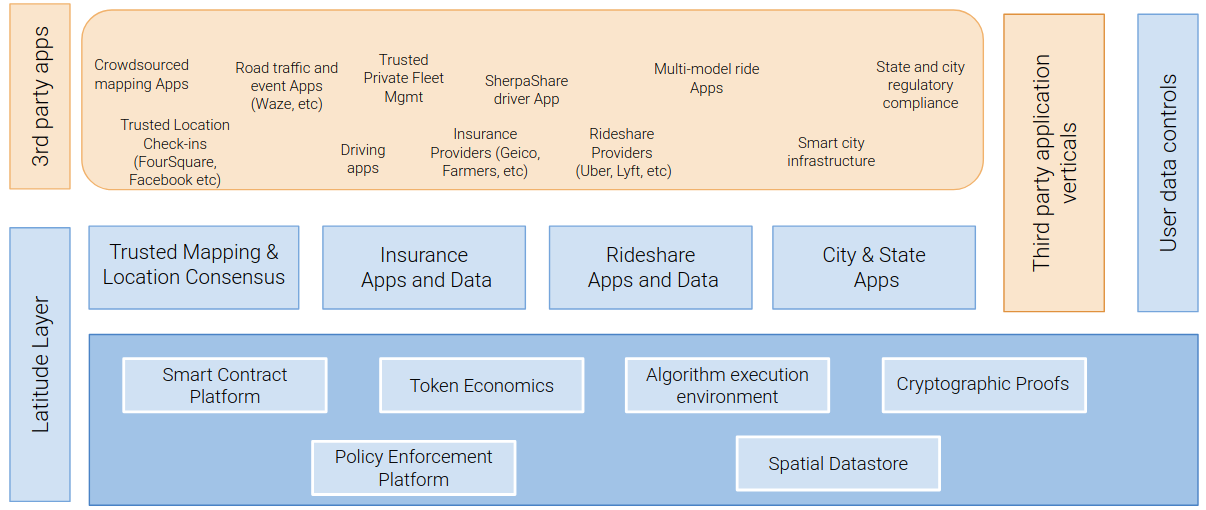
\includegraphics[width=0.90\textwidth]{latarch.png}
  \caption{Architecture of the Latitude Blockchain and associated platform ecosystem.}
    \label{fig:lat-arch}
\end{figure}

One of the central aspects of the Latitude blockchain is a geo-spatial datastore that fundamentally understands various
datatypes that are specific to transportation data. This datastore can use existing GIS databases that allow
de-centralized storage and access. The types of data include (i) georaphic data such as location (latitude, longitude),
(ii) mapping data such as roads, terrain, addresses, etc, (iii) sensor data such as driving data, driver score, miles
driven, route information, etc, (iv) multi-modal transport data such as biking, walking and other means of transport.
Each of these data types have very special characteristics which the underlying datastore can be optimized for and allow
for programming using what we call the {\em Latitude Smart Contract} framework. 

The datastore would include spatial, quad-tree or an R-tree based indexes for efficient querying and other operations that
most Geographic Information Systems (GIS) would support in a centralized manner today. It would also include functions
to compute heatmaps, driving maps and statistics such as Traffic predictions including real-time analytics. Depending on
how Latitude evolves, the datastore can include additional functionalities to support the data sharing among autonomous
vehicles since they use most of the similar datatypes mentioned above. The datastore would support circular, rectangular
and other range queries, K-nearest neighbor searches, route optimization algorithms, etc. Figure
\ref{fig:geo_spatial_query} shows some of the queries that such a datastore can support.

\begin{figure}[t]
    \centering
    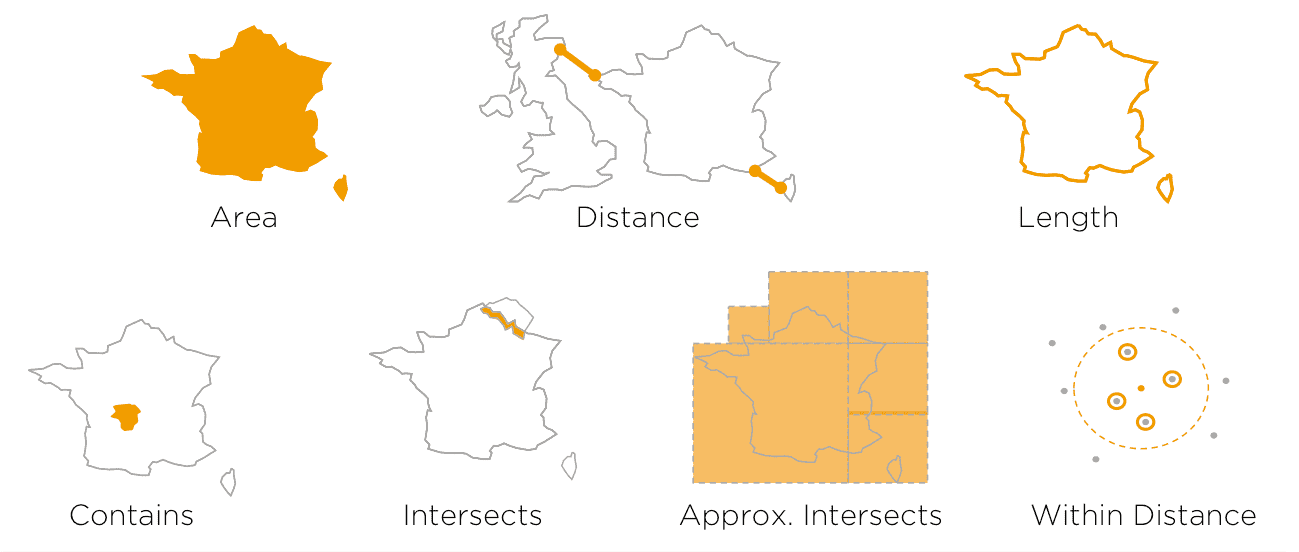
\includegraphics[width=0.90\textwidth]{geospatial_query.png}
  \caption{Examples of Geo-spatial queries that a spatial datastructure can support on the Latitude blockchain.}
    \label{fig:geo_spatial_query}
\end{figure}


Datastore
 - Optimized for Geographic, Geo-spatial data.
 - Location, Mapping data and computation.
 - Ability to Store, index, query and build smart contracts optimized for such data.
 - Support for various spatial indexes.
 - Location heatmaps.
 - Indexing road and driving data.
 - Primitives for storing driving data for autonomous vehicles

\noindent
{\textsf Strong crytographic foundation:}
Standard data encryption techniques allow for security guarantees in Latitude. Anonymity guarantees are provided using
privacy-preserving set operations such as given in \cite{kissner_set}, with suitable modifications to
anonymize spatial data which have user-location considerations \cite{divanis_kanon,xu_loc_anon}.
Cryptographic primitives for:
 - Security and privacy of data.
 - Anonymity guarantees using cryptographic set operations.
 - Enforcement of privacy when sharing data.
 - Sharing of “computation” instead of data when possible.
 - For eg: Sharing of DriverScore using a vetted algorithm.
 - Sharing proximity to a landmark instead of lat/lng.
 - Ability to find bad actors.
 - Detect privacy, anonymity and security violations.

\noindent
{\textsf Latitude Smart contract system:}

Smart contract system for Transportation applications.
 - Ability to convert “policies” such as GDPR into smart contract code.
 - Example, self destruct data after a time period.
 - Sandboxed trusted execution environment:
 - For algorithms:
   - DriverScore, Location heatmaps, Statistics.
   - Enforcing or verifying privacy and other govt policies/regulations.

Cryptographic proofs for applications:
 - Proof of Location. 
 - Proof of ride. 
 - Proof of mapping 
      (road/landmark exists or does not exist).
 - Proof of driver score 
 - Open, trusted, understood driver score computation algorithms.
 - Cryptographic proofs can be shared among entities, safely, securely.

\noindent
\subsection{Cryptoeconomics and Governance:}
Cryto-economics refers to the mechanics of the protocol underlying the blockchain operations which creates incentives
for the various stakeholders. For example, in the Latitude Blockchain it is possible to reward users for sharing their data
for certain purposes. For example, users can be rewarded if they share traffic data or accident information or better
routes. This is similar to the Waze model but creates legitimate rewards for users that have meaningful value outside
the Waze application. For an overview of cryptoeconomics in the blockchain space, please see \cite{sinclair_crypto}.

The core building block of the cryptoeconomics in Latitude is the Latitude Token, or LAT. This will be transacted in
each and every micro-transaction that takes place on the blockchain to create the right incentives, enforce smart
contracts and penalize Byzantine behavior. One of the fundamental design principles behind the protocol for the LAT
token is to create incentives assuming nodes are greedy and are interested in maximizing their gain. We will also build
safeguards against reasonable amount of collusion among nodes to subvert the system. The design is crafted such that the
best way for a node to maximize its revenue would be to participate with full honesty.

Latitude shall employ a Proof of Stake model (delegated or non-delegted) for particpation and core node-level mining. This mechanism has recently
gained popularity among a notable number of blockchains \cite{dpos_steemit}. This also allows for deposit slashing as a
technique to tackle Byzantine behavior. Latitude will employ techniques such as Minimal Slashing \cite{buterin_slashing}
for Byzantine fault tolerance and safety under distributed asynchronous operation.


Governance refers to a decentralized manner in which decisions are made using a consensus mechanism on the blockchain.
Decisions include basic constructs whether a node can join or leave the network. Or it can include key decisions on
whether an upgrade should be mandated on every node, a given participant such as a data provider should be penalized. It
could also include issues where humans get involved, such as when a user complains of a loss of privacy or a breach in
contract.

Recently blockchains have been moving towards governance using a small set of participants, such as trusted miners in
the case of Stellar and Ripple \cite{stellar_gateway}. The EOS blockchain uses a similar concept of a core set of block
producers who are elected based on a nomination and voting process \cite{eos_producers}. For discussion around
Governance in Ethereum, refer to \cite{buterin_gov}. Latitude uses a similar concept of a {\em council} of participants.
These are entities (nodes or organizations) that have demonstrated participating using earned trust through honest
operation, accumulating stake, demonstrated good intent and establishing trust. Some members of this council might
include the core Latitude developers which allows them to implement operations such as updates, bug fixes and so on. The
council members shall be elected using the an election protocol on the blockchain. It might be possible to directly
nominate certain council members such as regulatory bodies who have general interest in user rights, privacy and
enforcement. 

 - Crypto-incentives for honest operation.
 - Penalties for malicious intent.
 - Governance based on consensus and roles using a council.
 - Council members elected using voting, stake and established trust.
 - Some council members can have restricted access.
 - Eg: US govt can have voting rights on US data/users, etc.

User incentives:
 - Users have full control over their data and computation.
 - Users can issue or request proofs to carry over to other applications.
 - User’s have incentive to share data, participate in improving the common denominator.
 - Malicious intent, Byzantine behavior.
   - Can be detected using a combination of consensus and incentives.
   - Best interest of users to act honestly by design.


\noindent
{\textsf Performance considerations:}
Performance:
- Transaction speed. Data throughput. Storage capabilities.


-----------------------------------------------------------------------------
%  BIBLIOGRAPHY
%-----------------------------------------------------------------------------
\section{References}
\bibliography{latitude.bib}

\end{document}
